\documentclass[11pt,letterpaper]{article}

%%%%%%%%%%%%%%%%%%%%%%%%%%%%%%%%%%%
% IMPORTACIÓN DE CONFIGURACIONES
%%%%%%%%%%%%%%%%%%%%%%%%%%%%%%%%%%%

\input{configuracion}

%%%%%%%%%%%%%%%%%%%%%%%%%%%%
% INICIO DE DOCUMENTO
%%%%%%%%%%%%%%%%%%%%%%%%%%%%

\begin{document}

%%%%%%%%%%%%%%%%%%%%%%%%%%%%
% ENCABEZADO
%%%%%%%%%%%%%%%%%%%%%%%%%%%%
\begin{center}
    \begin{minipage}{3cm}
    	\begin{center}
    		
\includegraphics[height=3.4cm]{Logo_UNAM.png}
    	\end{center}
    \end{minipage}\hfill
    \begin{minipage}{10cm}
    	\begin{center}
    	\textbf{\large Universidad Nacional Autónoma de México}\\[0.1cm]
        \textbf{Facultad de Ciencias}\\[0.1cm]
        \textbf{Geometría Analítica II $|$ Grupo 4092}\\[0.1cm]
        Quizz 3\\[0.1cm]
        Martínez Castro Alvaro Leonardo\\[0.1cm]
        \today
    	\end{center}
    \end{minipage}\hfill
    \begin{minipage}{3cm}
    	\begin{center}
    		
\includegraphics[height=3.4cm]{Logo_FC.png}
    	\end{center}
    \end{minipage}
\end{center}

\rule{17cm}{0.1mm}

%%%%%%%%%%%%%%%%%%%%%%%%%%%%
% FIN DE ENCABEZADO
%%%%%%%%%%%%%%%%%%%%%%%%%%%%

\begin{inciso}{Banda de Möbius}
- La banda de Möbius es una superficie dada por la parametrización:
\[
\varphi(t, s) = \left((1 + s \cos t) \cos(2t), \, (1 + s \cos t) \operatorname{sen}(2t), \, s \operatorname{sen}t\right), \quad \text{con } t \in [0, 2\pi] \; \text{y} \; s \in \left[-\frac{1}{2}, \frac{1}{2}\right].
\]

Prueba que en cada punto existe un segmento de recta que está totalmente contenida en la superficie. Esboza la gráfica de esta superficie.

\begin{problema}{Banda de Möbius}
- Notemos que la parametrización se puede reescribir de la forma
\[
\varphi(t,s) = \big(\cos(2t),\sin(2t),0\big) + s\,\big(\cos t\cos(2t),\, \cos t\sin(2t),\, \sin t\big),
\]
ya que
\[
(1+s\cos t)\cos(2t)=\cos(2t)+s\cos t\cos(2t) \quad\text{y}\quad (1+s\cos t)\sin(2t)=\sin(2t)+s\cos t\sin(2t).
\]

Podemos observar que para cada valor fijo de \(t\), la función
\[
s\mapsto \varphi(t,s)
\]
es una aplicación afín en \(s\) (es decir, una recta en \(\mathbb{R}^3\)). Específicamente, si fijamos \(t_0\), tenemos
\[
\varphi(t_0,s) = \gamma(t_0) + s\,v(t_0),
\]
donde
\[
\gamma(t_0) = \big(\cos(2t_0),\,\sin(2t_0),\,0\big) \quad \text{y} \quad v(t_0) = \big(\cos t_0\cos(2t_0),\, \cos t_0\sin(2t_0),\, \sin t_0\big).
\]
Esto significa que, para cada \(t_0\), la imagen de \(\varphi(t_0,s)\) (con \(s\in \left[-\tfrac12,\tfrac12\right]\)) es un segmento de recta contenido en la banda de Möbius.

Dado que cada punto \(p\) de la superficie tiene la forma \(p=\varphi(t_0,s_0)\) para algún \(t_0\) y \(s_0\), concluimos que \(p\) está sobre el segmento
\[
\{\varphi(t_0,s) : s \in \left[-\tfrac12,\tfrac12\right]\},
\]
el cual está totalmente contenido en la superficie.

Así, se ha probado que en cada punto de la banda de Möbius existe un segmento de recta que está completamente contenido en ella. 

\begin{figure}[H]
    \centering
    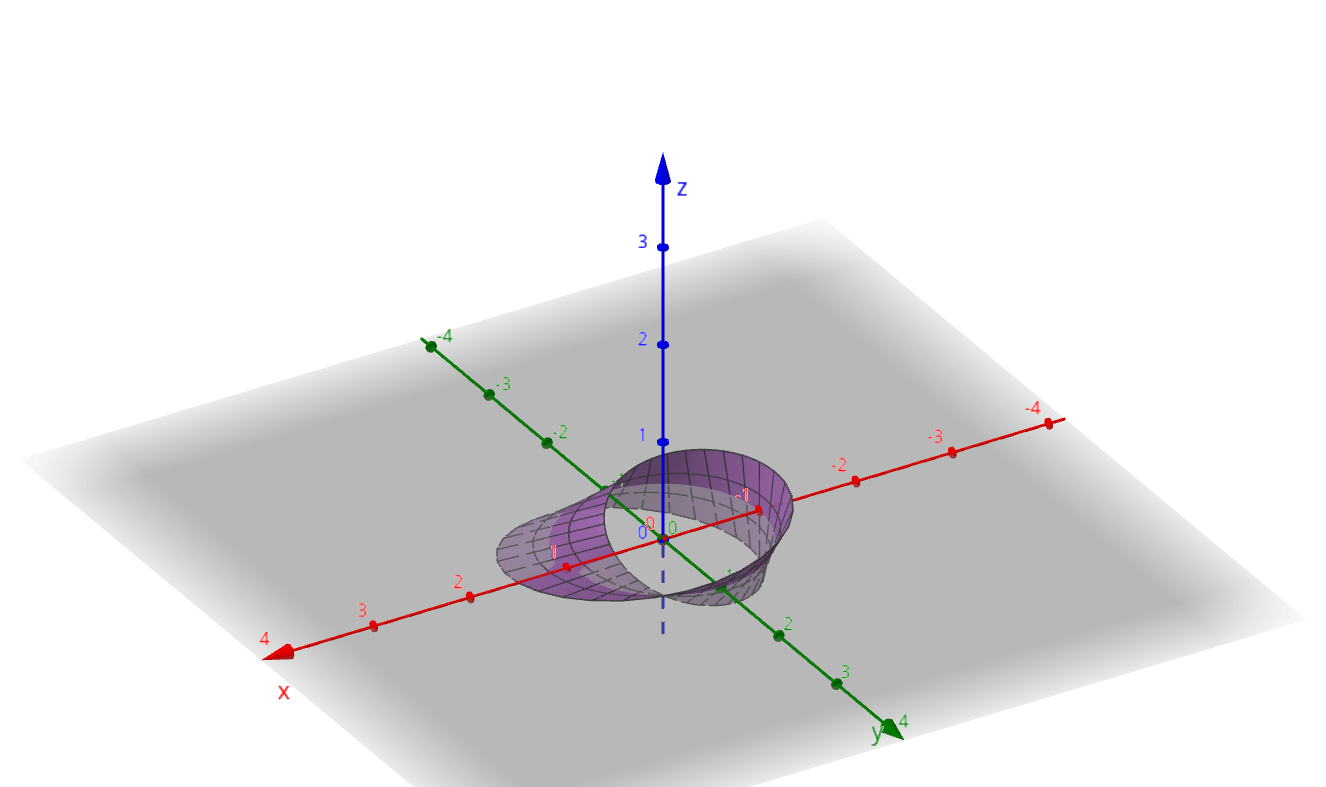
\includegraphics[height=6cm]{BandaMoebius.png}
\end{figure}
\end{problema}

\end{inciso}

\begin{inciso}{Cilindro circular}
- Muestra que el cilindro circular es el lugar geométrico de puntos en el espacio cuya distancia a una recta es constante.
\begin{problema}{Cilindro circular}
- Supongamos que la recta \( L \) coincide con el eje \( z \). Esto simplifica los cálculos sin pérdida de generalidad, ya que cualquier recta en el espacio puede trasladarse o rotarse a esta posición.\\
Sea \( P = (x, y, z) \) un punto cualquiera en el espacio. La distancia de \( P \) al eje \( z \) (la recta \( L \)) está dada por:
\[
d(P, L) = \sqrt{x^2 + y^2}.
\]

Si \( d(P, L) = r \) (constante), entonces:
\[
\sqrt{x^2 + y^2} = r \quad \implies \quad x^2 + y^2 = r^2.
\]
Esta es la ecuación de un \textbf{cilindro circular recto} de radio \( r \), cuyo eje es \( L \) (el eje \( z \)).

Si \( L \) es una recta arbitraria en el espacio, se puede elegir un sistema de coordenadas donde \( L \) coincida con el eje \( z \) mediante rotaciones y traslaciones. La ecuación \( x^2 + y^2 = r^2 \) seguirá representando un cilindro circular de radio \( r \), pero ahora con eje en \( L \).

Ahora bien, podemos interpretar geométricamente lo siguiente: 

\begin{itemize}
    \item Todos los puntos \( (x, y, z) \) que satisfacen \( x^2 + y^2 = r^2 \) están a distancia \( r \) del eje \( z \).
    \item Al variar \( z \), el cilindro se extiende infinitamente en ambas direcciones a lo largo de \( L \).
\end{itemize}

Si \( L \) es el eje \( z \), el cilindro correspondiente es:
\[
x^2 + y^2 = r^2, \quad z \in \mathbb{R}.
\]
Para cualquier punto \( (x, y, z) \) en esta superficie, su distancia al eje \( z \) es siempre \( r \).
\\\\
El cilindro circular es precisamente el conjunto de puntos en el espacio cuya distancia a una recta \( L \) es constante. Esto se cumple tanto para el caso particular (eje \( z \)) como para cualquier recta en el espacio, gracias a la invariancia de la distancia bajo movimientos rígidos (rotaciones y traslaciones).
\end{problema}

\end{inciso}

\end{document}


    